\mainmatter
\pagestyle{headings}
\chapter{Research}
\label{ch:research}

\section{Analysis}
The whole data set and data analysis script can be found on the GitHub repository\footnote{https://github.com/MoutPessemier/A-Survey-On-The-Impact-of-Customer-Chatbots-on-E-commerce}.\\
\break
The data has been anonimised in Excel. A new column was created called 'taskCategory'. The tasks performed are categorised in one of the following 4 categories:
\begin{itemize}
	\item FAQ
	\item Personalised question
	\item Complaint
	\item Sales
\end{itemize}
From the 63 entries, we had to throw 5 away:
\begin{itemize}
	\item 3 because of the used chatbot: they were no telecom chatbots.
	\item 1 entry was a duplicate.
	\item 1 entry responded with one answer only (only yes and only neutral in part 2)
\end{itemize}

\subsection{Environment Variables}
\subsubsection{Age}
% amai das echt brak geschreven, nog is nadenken hoe dit moet geschreven worden
The age variable has an overall mean value of 26,36 and a standard deviation of 7,60. If age gets grouped by the different providers, the following is plotted. Next to the plot, there is a frequency table that shows the different ages appearing in this survey, ordered from most common to least common.
\begin{figure}[!htb]
	\minipage{0.75\textwidth}
	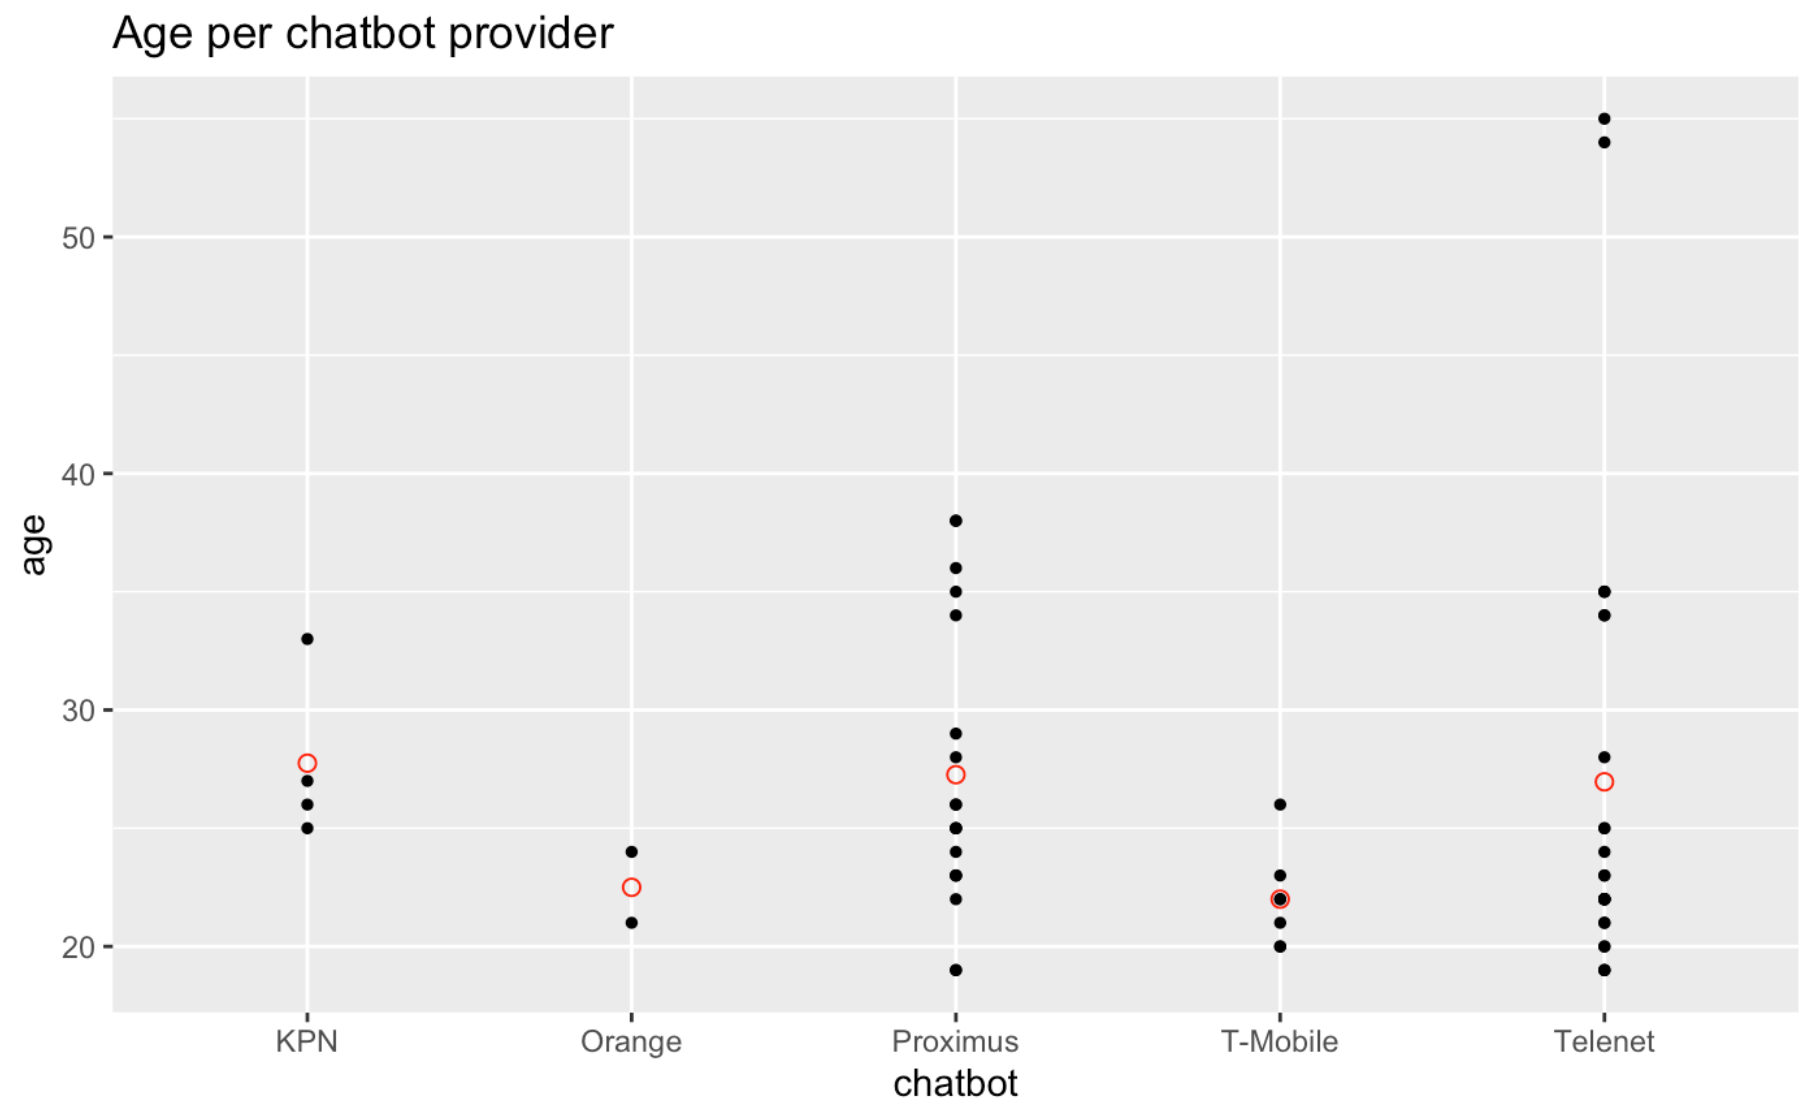
\includegraphics[width=\linewidth]{../LaTeX/Figures/Environments/AgePlot.png}
	\caption{The distribution of the age variable per chatbot provider.}\label{fig:agePlot}
	\endminipage\hfill
	\minipage{0.24\textwidth}
	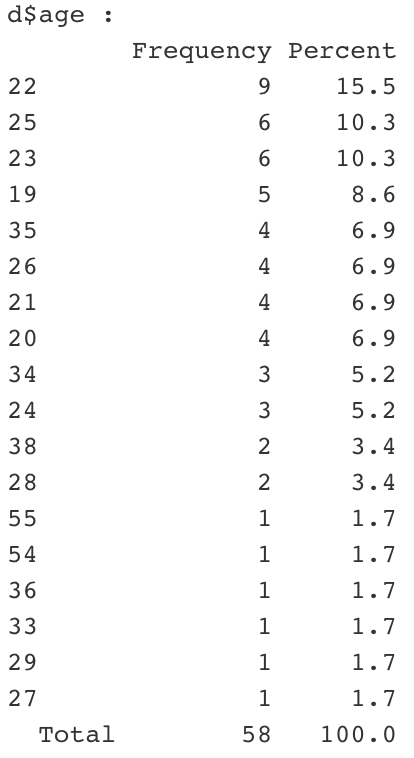
\includegraphics[width=\linewidth]{../LaTeX/Figures/Environments/AgeFreq.png}
	\caption{A frequency table of all the entries' ages.}\label{fig:ageFreq}
	\endminipage\hfill
\end{figure}

\subsubsection{Highest degree}
Looking at the acquired degrees of the respondents, most of them (19) have a master degree, followed by an academic bachelor (16).
\begin{figure}[!htb]
	\minipage{0.55\textwidth}
	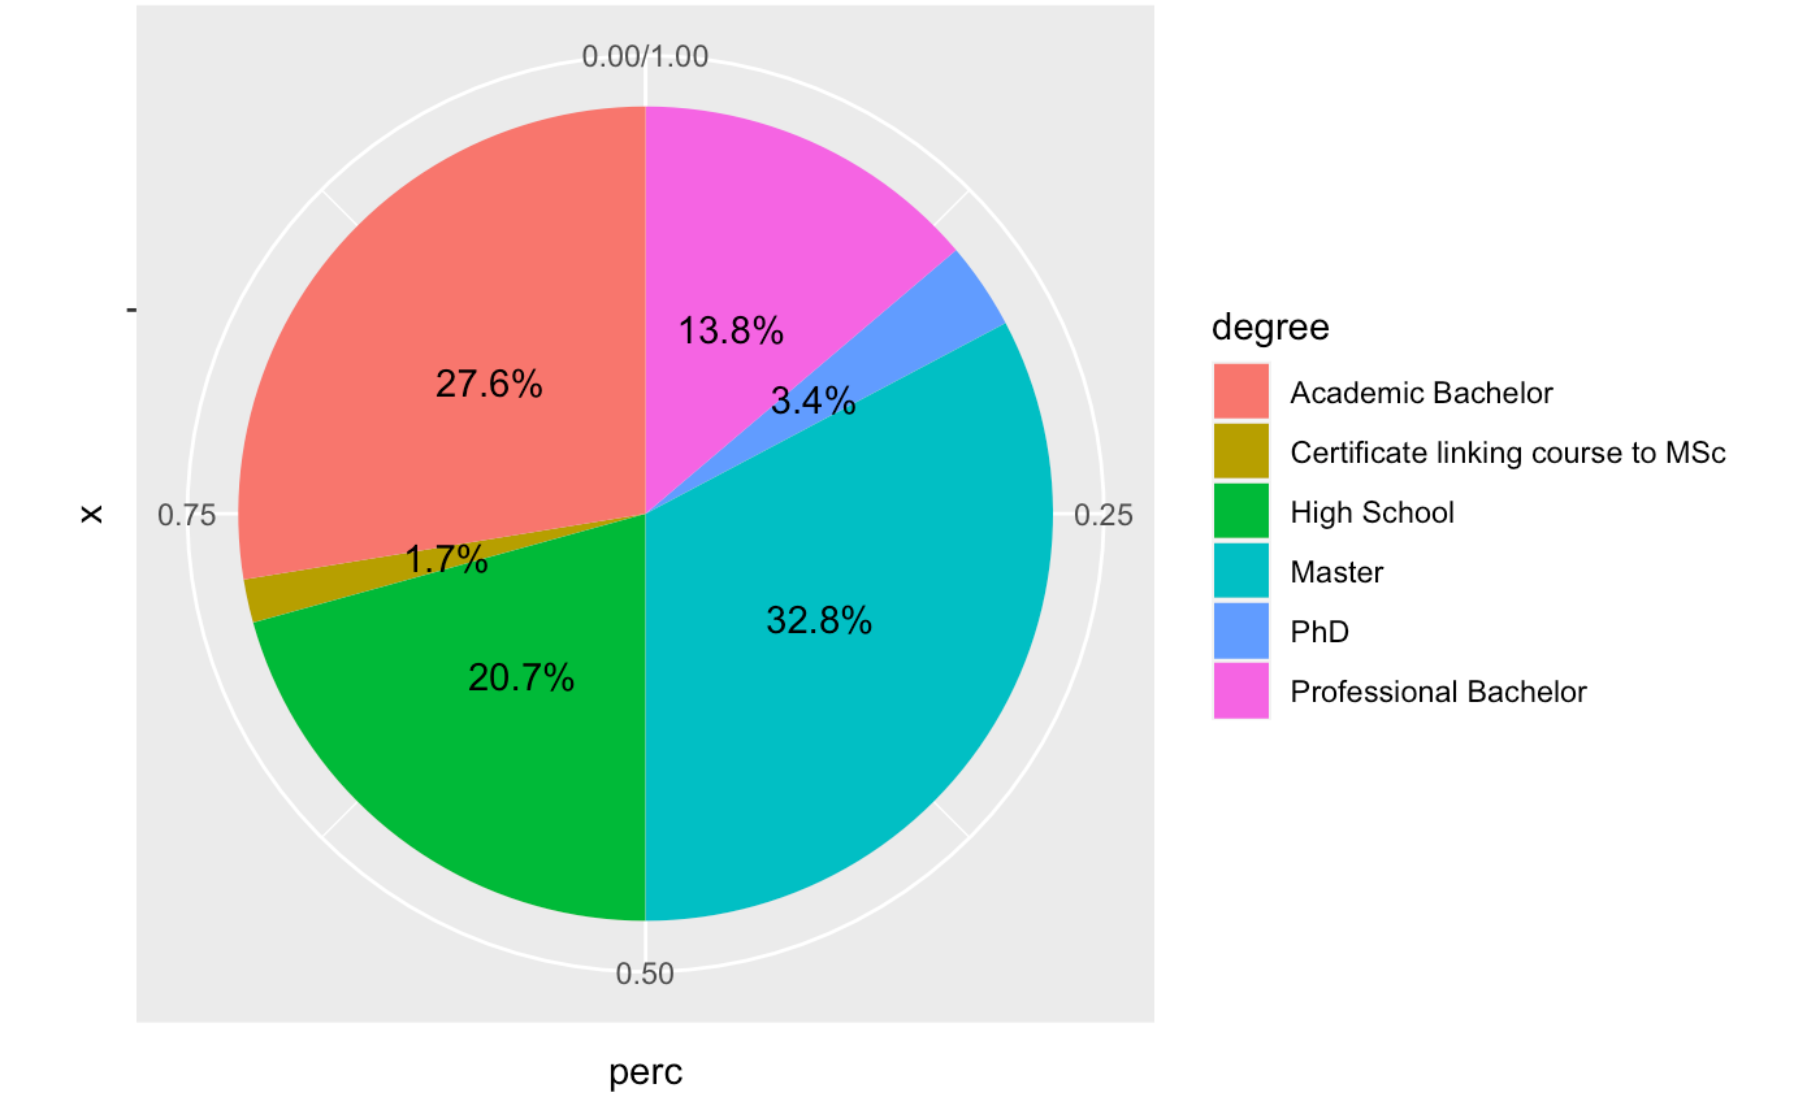
\includegraphics[width=\linewidth]{../LaTeX/Figures/Environments/DegreePlot.png}
	\caption{The distribution of the degree variable.}\label{fig:degreePlot}
	\endminipage\hfill
	\minipage{0.44\textwidth}
	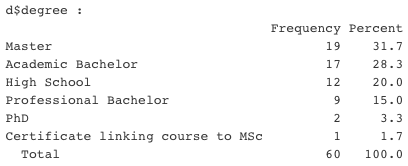
\includegraphics[width=\linewidth]{../LaTeX/Figures/Environments/DegreeFreq.png}
	\caption{A frequency table of all the entries' degrees.}\label{fig:degreeFreq}
	\endminipage\hfill
\end{figure}

\subsubsection{Gender}
There were more male respondents than female respondents. The difference between the two is 9. There was also one non-binary respondent.
\begin{figure}[!htb]
	\minipage{0.69\textwidth}
	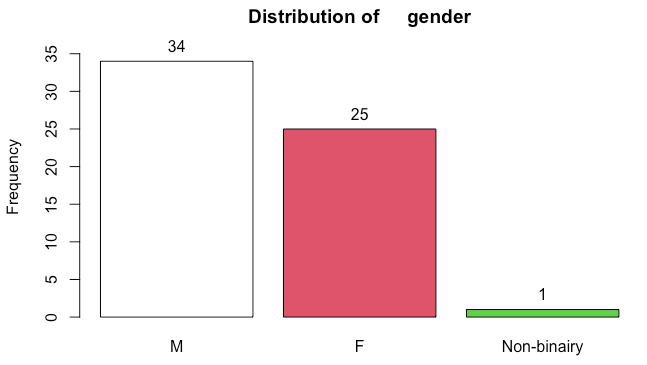
\includegraphics[width=\linewidth]{../LaTeX/Figures/Environments/GenderPlot.png}
	\caption{The distribution of the gender variable.}\label{fig:genderPlot}
	\endminipage\hfill
	\minipage{0.30\textwidth}
	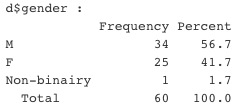
\includegraphics[width=\linewidth]{../LaTeX/Figures/Environments/GenderFreq.png}
	\caption{A frequency table of all the entries' genders.}\label{fig:genderFreq}
	\endminipage\hfill
\end{figure}

\subsubsection{Company of chatbot}
Telenet has the most respondents, followed closly by Proximus. The other chatbot providers are less represented. 
\begin{figure}[!htb]
	\minipage{0.69\textwidth}
	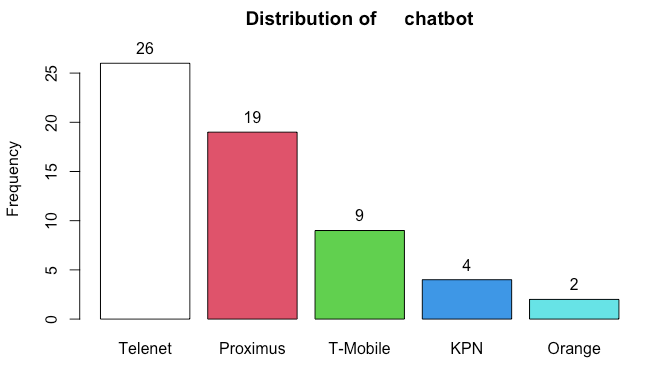
\includegraphics[width=\linewidth]{../LaTeX/Figures/Environments/ChatbotPlot.png}
	\caption{The distribution of the different chatbot providers and the amount of respondents for each provider.}\label{fig:chatbotPlot}
	\endminipage\hfill
	\minipage{0.30\textwidth}
	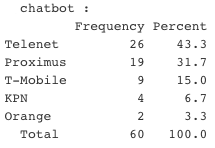
\includegraphics[width=\linewidth]{../LaTeX/Figures/Environments/ChatbotFreq.png}
	\caption{A frequency table of all the entries' used chatbots.}\label{fig:chatbotFreq}
	\endminipage\hfill
\end{figure}

\subsubsection{Used language}
Most users used Dutch as their preferred language of interaction which doesn't come as a surprise since this thesis focuses on the Flemish part of Belgium along with the Netherlands. Afterwards, Egnlish was the second most used language and French came last.
\begin{figure}[!htb]
	\minipage{0.69\textwidth}
	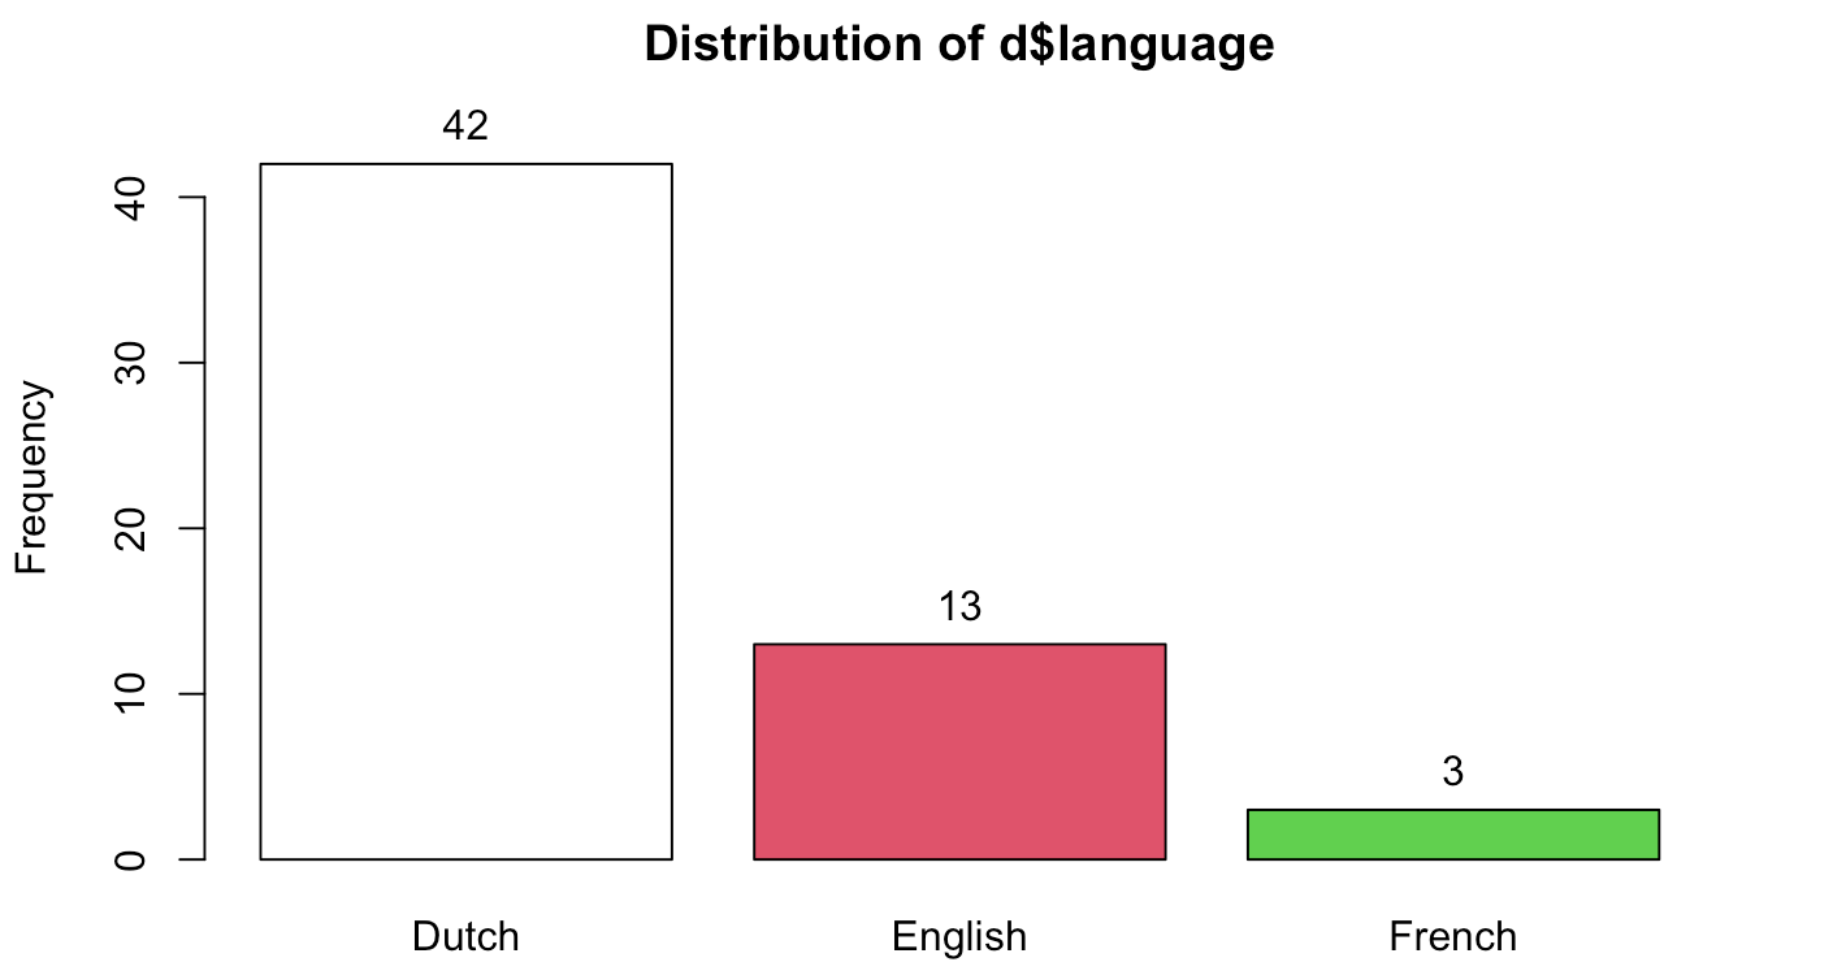
\includegraphics[width=\linewidth]{../LaTeX/Figures/Environments/LanguagePlot.png}
	\caption{The distribution of the language variable.}\label{fig:languagePlot}
	\endminipage\hfill
	\minipage{0.30\textwidth}
	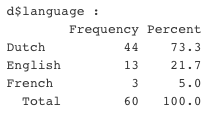
\includegraphics[width=\linewidth]{../LaTeX/Figures/Environments/LanguageFreq.png}
	\caption{A frequency table of all the entries' used languages.}\label{fig:languageFreq}
	\endminipage\hfill
\end{figure}

\subsubsection{Platform}
Most chatbots were used on the website of the provider themselves. Only a small percentage were used in app or via Facebook Messenger.
\begin{figure}[!htb]
	\minipage{0.69\textwidth}
	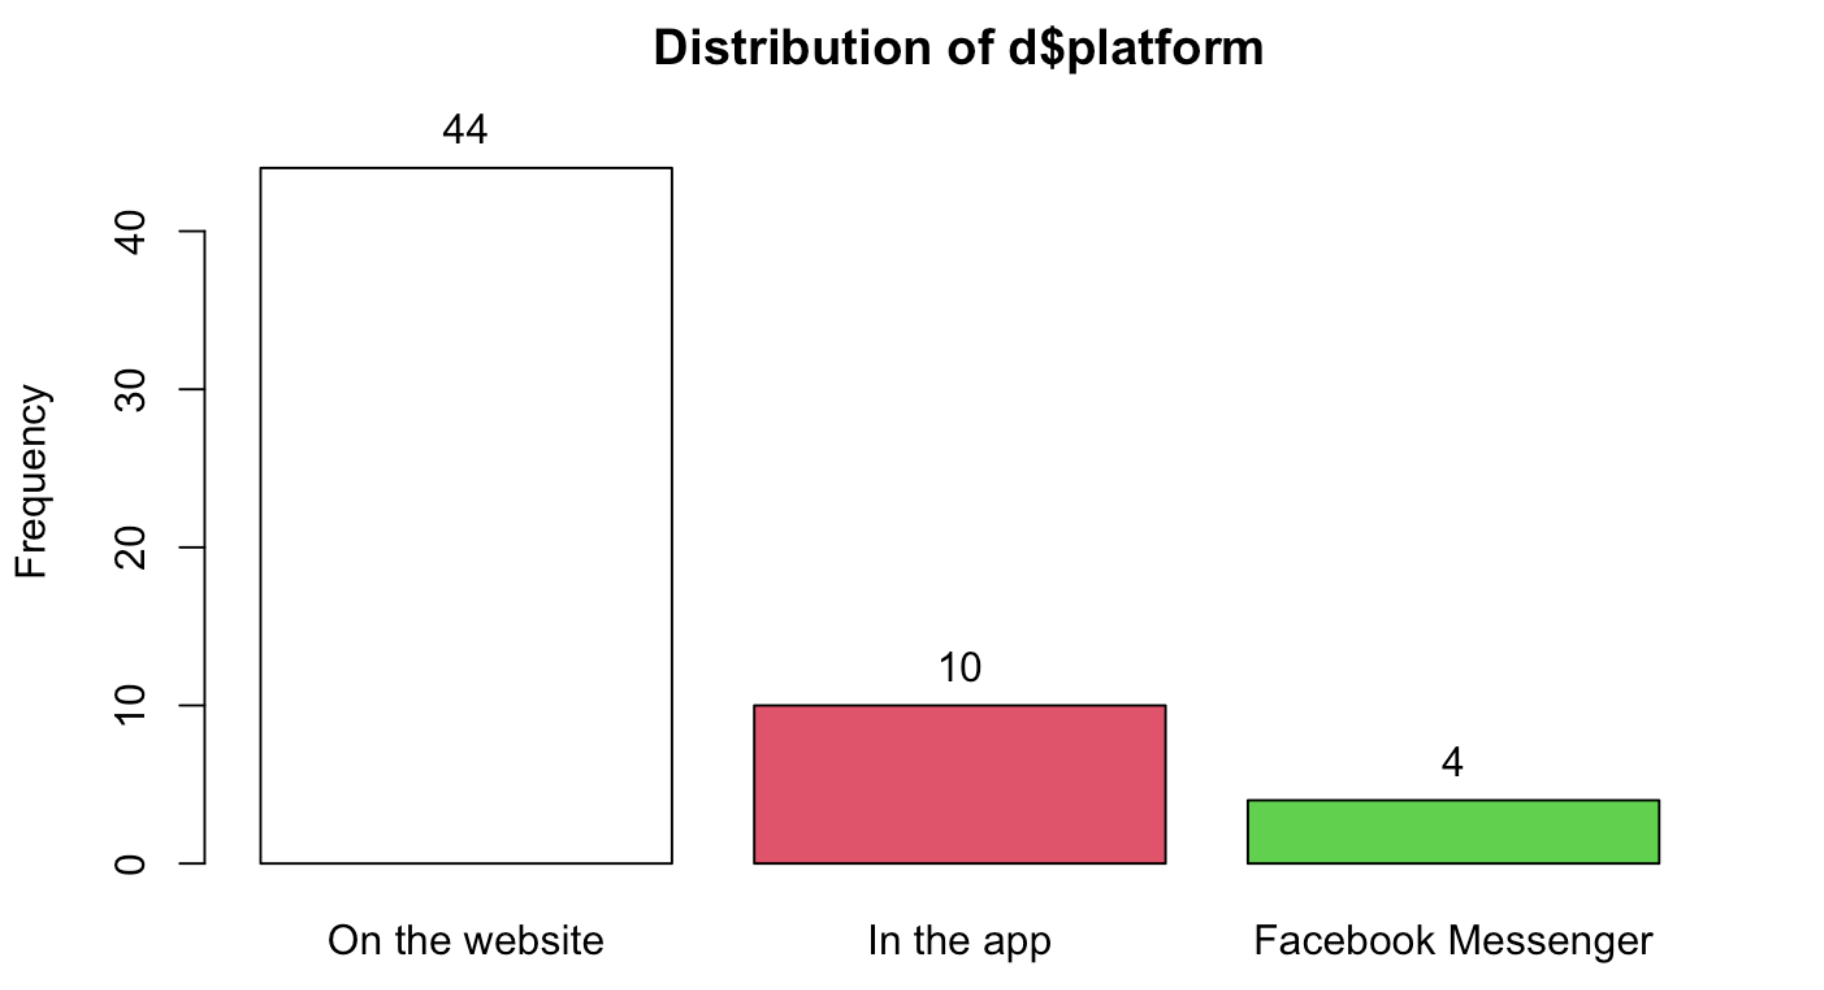
\includegraphics[width=\linewidth]{../LaTeX/Figures/Environments/PlatformPlot.png}
	\caption{The distribution of the platform variable.}\label{fig:platformPlot}
	\endminipage\hfill
	\minipage{0.30\textwidth}
	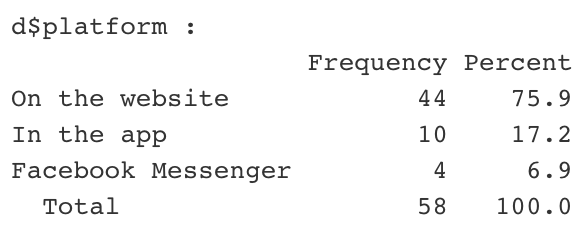
\includegraphics[width=\linewidth]{../LaTeX/Figures/Environments/PlatformFreq.png}
	\caption{A frequency table of all the entries' used platform to interact with the chatbot.}\label{fig:platformFreq}
	\endminipage\hfill
\end{figure}

\subsection{Comparative Study}
\subsubsection{Business view (interviews)}
% Elk belangrijk stuk van het interview beschrijven per puntje, elk bedrijf telkens bespreken

\subsubsection{Customer view (survey)}
%Dit moeten we bespreken met Etikala

\subsection{Importance Study - Kano}
\subsubsection{Discrete analysis}
% Stuk met tabel waar alles is verdeeld (kijk naar thesis ugent)
To start with the KANO analysis, there first had to be made a clear mapping between the functional and dysfunctional question and which label of KANO would be assigned to the outcome of this mapping. The mapping can be found in Figure \ref{fig:kanoOverview}.
\begin{figure}[htb!]
	\centering
	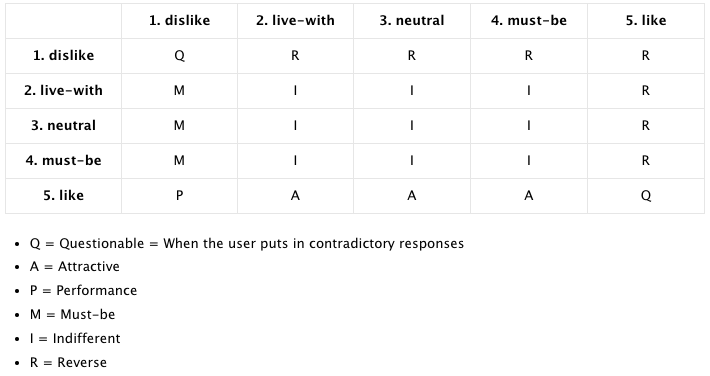
\includegraphics[width=\linewidth]{../LaTeX/Figures/Kano/KANOOverview.png}
	\caption{The mapping between the functional and dysfunctional question and the KANO label associated.}
	\label{fig:kanoOverview}
\end{figure}
\break
\break
Afterwards, for each scenario as well as the general questions of the survey, the answers were counted and added per label. The highest label was assigned. If there was an overlap between two or more labels, the label with the most impact was chosen. An overview  of the label assigned to each entry can be found in Figure \ref{fig:kanoTable}
\begin{figure}[!htb]
	\centering
	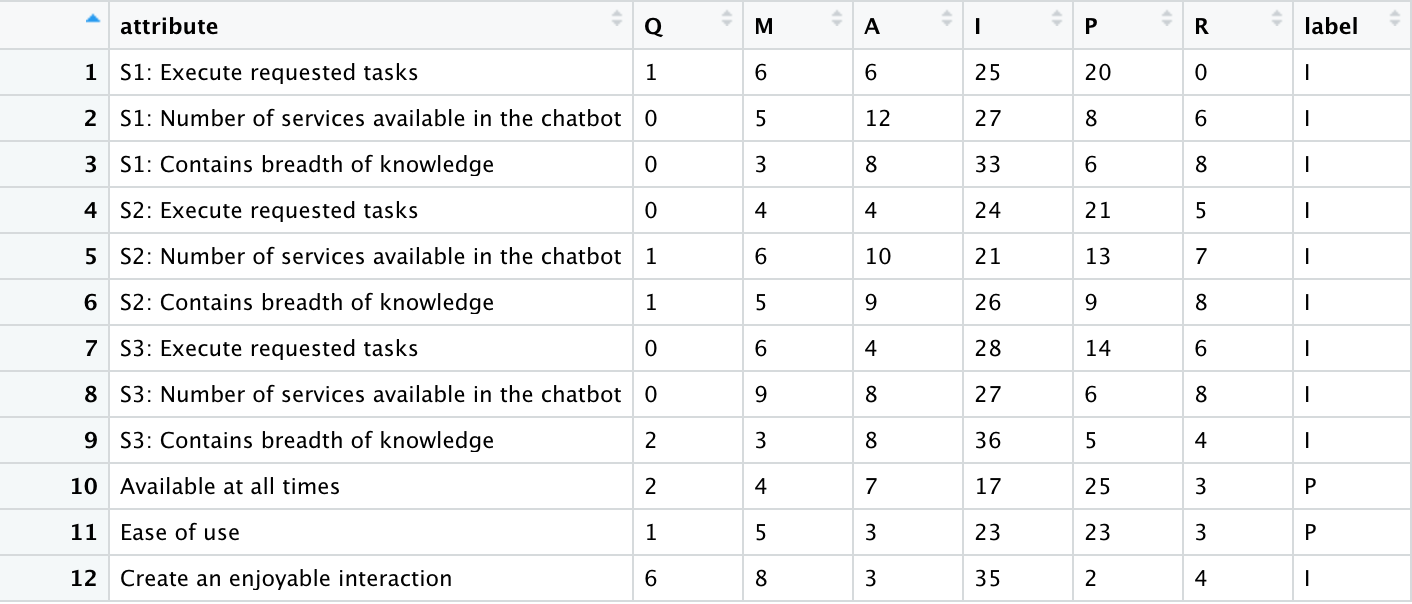
\includegraphics[width=\linewidth]{../LaTeX/Figures/Kano/KanoTable.png}
	\caption{Each entry with it's assigned KANO label.}
	\label{fig:kanoTable}
\end{figure}
\subsubsection{Continuous analysis}
% Stuk met grafiek waar de verschillende attributes zijn opgesteld volgens hun categorie (kijk naar thesis ugent)
Now that each entry has a label assigned to it and for every entry, the different categories are counted. Based on this, both the satisfaction as well as the dissatisfaction coefficient can be calculated. The calculations can be seen in Figure \ref{fig:satisfactionCoef} and Figure \ref{fig:dissatisfactionCoef}.
\begin{figure}[!htb]
	\centering
	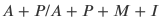
\includegraphics{../LaTeX/Figures/Kano/SatisfactionCoef.png}
	\caption{The satisfaction coefficient.}
	\label{fig:satisfactionCoef}
\end{figure}
\begin{figure}[!htb]
	\centering
	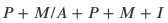
\includegraphics{../LaTeX/Figures/Kano/DissatisfactionCoef.png}
	\caption{The dissatisfaction coefficient.}
	\label{fig:dissatisfactionCoef}
\end{figure}
\break
After calculating both these scores for each entry, they were plotted in  a scatterplot, dividing them up into one of the four main categories of KANO. The categorisation can be found in Figure \ref{fig:satisfactionPlot}
\begin{figure}[!htb]
	\centering
	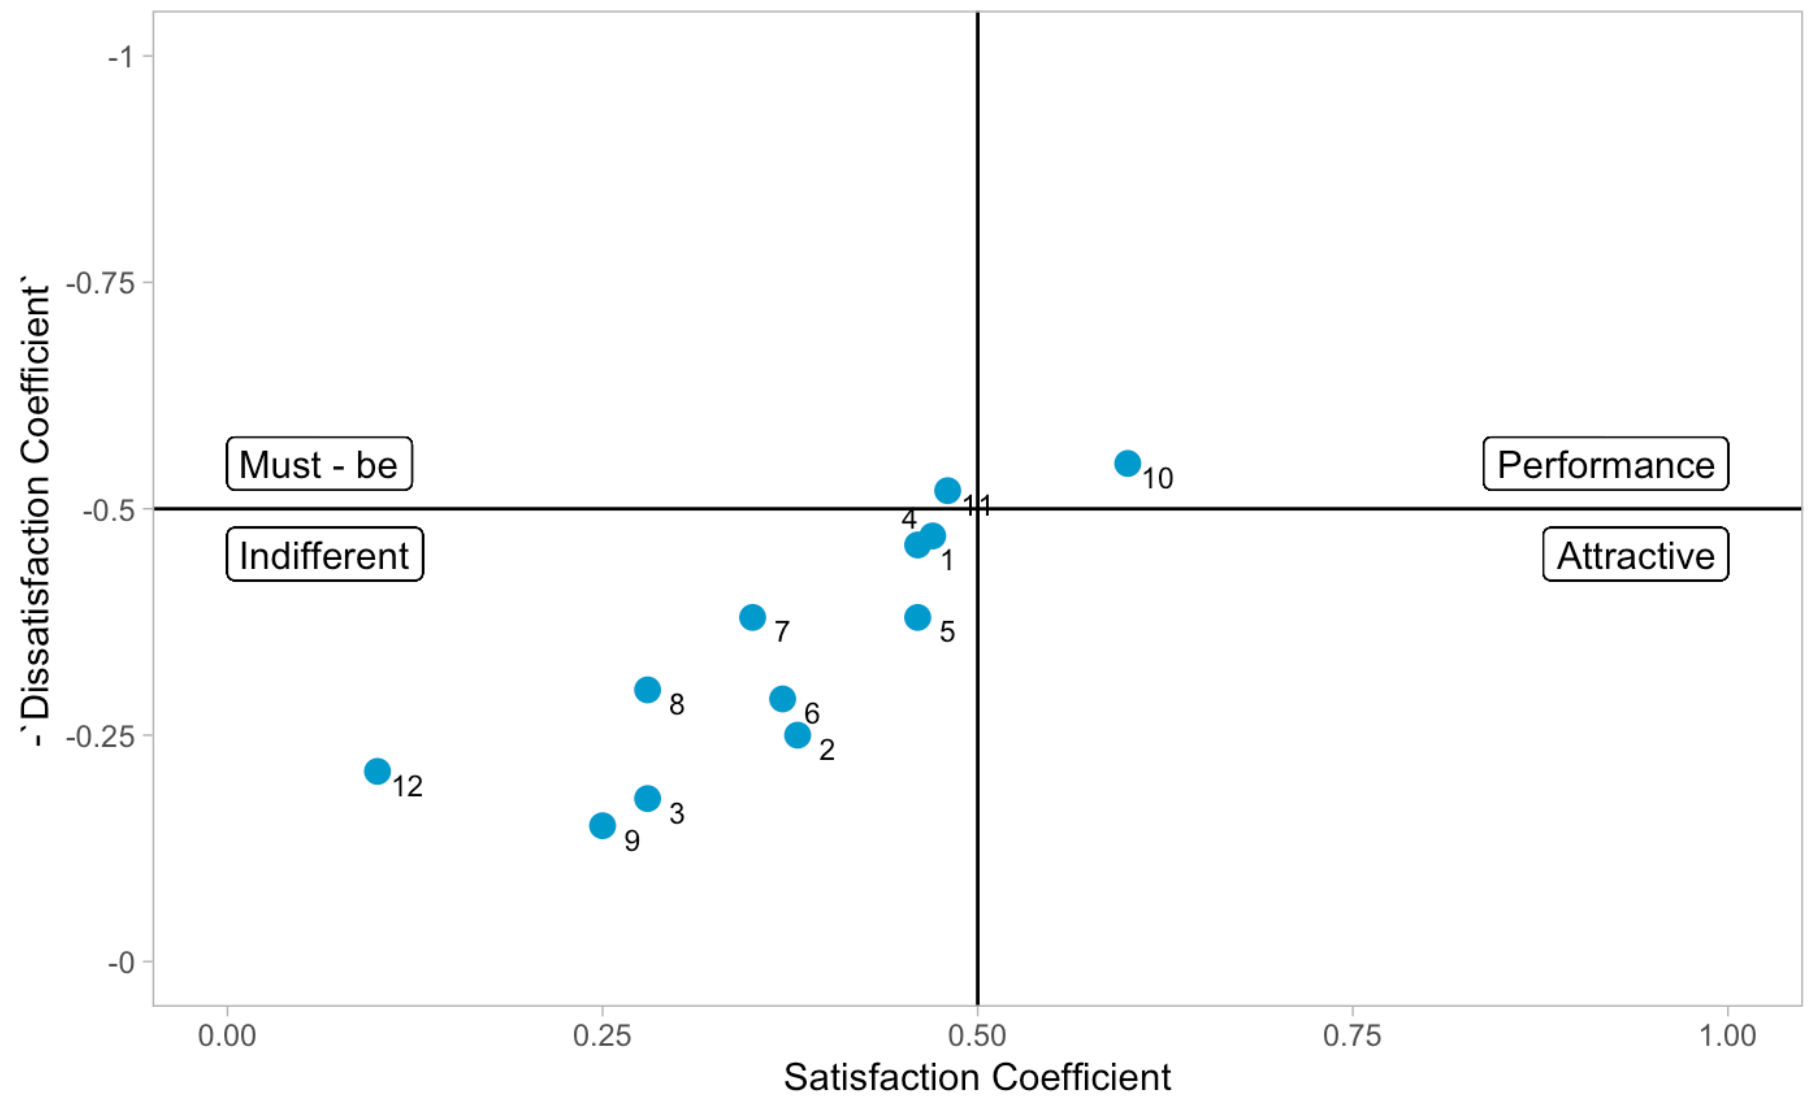
\includegraphics[width=\linewidth]{../LaTeX/Figures/Kano/SatisfactionPlot.png}
	\caption{The satisfaction/dissatisfaction plot.}
	\label{fig:satisfactionPlot}
\end{figure}

\section{Discussion}
%HIER MOETEN WE OP DE HYPOTHESES ANTWOORDEN!!!!

\subsection{The future vision of telecom chatbots}
%Wat hebben de bedrijven gezegd over de toekomst van de chatbots?

\subsection{Quality attributes for telecom chatbots}
% hier zou ik een overzichtstabel zetten van de verschillende attributen die we uit de vragen hebben gehaald
